\documentclass[11pt,a4paper,oneside]{book}

% ------------------------------------------------------------------
%  Codificação e idioma
% ------------------------------------------------------------------
\usepackage[utf8]{inputenc}
\usepackage[T1]{fontenc}
\usepackage[brazil]{babel}
\usepackage{lmodern}

% ------------------------------------------------------------------
%  Matemática
% ------------------------------------------------------------------
\usepackage{amsmath,amssymb,amsthm,mathtools}
\usepackage{bm}

% ------------------------------------------------------------------
%  Figuras, tabelas e layout
% ------------------------------------------------------------------
\usepackage{graphicx}
% Busca as figuras primeiro na subpasta local "figs/" (cópia autocontida) e,
% caso não exista, nas pastas de imagens compartilhadas dos slides — mesma
% convenção usada pelos slides da disciplina (../images).
\graphicspath{{figs/}{../images/}{../../images/}}
\usepackage{float}
\usepackage{booktabs}
\usepackage{array}
\usepackage{caption}
\usepackage{subcaption}
\captionsetup{font=small,labelfont=bf}
\usepackage[dvipsnames,table]{xcolor}
\usepackage[a4paper,margin=2.7cm,headheight=14pt]{geometry}
\usepackage{microtype}
\usepackage{enumitem}
\usepackage{listings}
\usepackage{fancyhdr}
\usepackage{emptypage}

% ------------------------------------------------------------------
%  Hyperref (por último)
% ------------------------------------------------------------------
\usepackage[hidelinks,colorlinks=true,linkcolor=MidnightBlue,
            citecolor=MidnightBlue,urlcolor=RoyalBlue]{hyperref}

% ------------------------------------------------------------------
%  Cores do livro
% ------------------------------------------------------------------
\definecolor{corcap}{RGB}{20,60,110}
\definecolor{corbox}{RGB}{240,244,250}
\definecolor{corboxb}{RGB}{20,60,110}
\definecolor{corcode}{RGB}{248,248,248}

% ------------------------------------------------------------------
%  Ambientes de teorema (notação formal)
% ------------------------------------------------------------------
\theoremstyle{definition}
\newtheorem{definicao}{Definição}[chapter]
\newtheorem{exemplo}{Exemplo}[chapter]
\newtheorem{observacao}{Observação}[chapter]

\theoremstyle{plain}
\newtheorem{teorema}{Teorema}[chapter]
\newtheorem{proposicao}{Proposição}[chapter]
\newtheorem{corolario}{Corolário}[chapter]
\newtheorem{lema}{Lema}[chapter]

\renewcommand{\qedsymbol}{$\blacksquare$}

% Caixa de destaque para resultados-chave
\usepackage[most]{tcolorbox}
\usepackage{empheq}
\newtcolorbox{destaque}[1][]{
  colback=corbox, colframe=corboxb, boxrule=0.6pt, arc=2pt,
  left=6pt,right=6pt,top=5pt,bottom=5pt, #1}

% --- Caixas de destaque para os ambientes de teorema ---
\definecolor{corplain}{RGB}{20,60,110}   % azul (teorema/proposição/...)
\definecolor{cordef}{RGB}{110,80,20}     % âmbar (definição/exemplo/...)
\tcbset{
  thmplain/.style={breakable, enhanced, arc=2pt, boxrule=0.4pt,
    colback=corplain!5, colframe=corplain, left=8pt, right=8pt,
    top=5pt, bottom=5pt, borderline west={2.5pt}{0pt}{corplain}},
  thmdef/.style={breakable, enhanced, arc=2pt, boxrule=0.4pt,
    colback=cordef!6, colframe=cordef!85!black, left=8pt, right=8pt,
    top=5pt, bottom=5pt, borderline west={2.5pt}{0pt}{cordef!85!black}},
}
\tcolorboxenvironment{teorema}{thmplain}
\tcolorboxenvironment{proposicao}{thmplain}
\tcolorboxenvironment{corolario}{thmplain}
\tcolorboxenvironment{lema}{thmplain}
\tcolorboxenvironment{definicao}{thmdef}
\tcolorboxenvironment{exemplo}{thmdef}
\tcolorboxenvironment{observacao}{thmdef}

% --- Caixa para equações principais ---
% Uso: \begin{empheq}[box=\tcbhighmath]{equation} ... \end{empheq}
\tcbset{highlight math style={enhanced, colback=corplain!7,
  colframe=corplain, boxrule=0.5pt, arc=2pt,
  left=3pt, right=3pt, top=2pt, bottom=2pt}}

% ------------------------------------------------------------------
%  Cabeçalhos
% ------------------------------------------------------------------
\pagestyle{fancy}
\fancyhf{}
\renewcommand{\headrulewidth}{0.4pt}
\fancyhead[L]{\small\itshape SEL0359 -- Controle Digital}
\fancyhead[R]{\small\itshape\nouppercase{\leftmark}}
\fancyfoot[C]{\thepage}

% ------------------------------------------------------------------
%  Estilo de código (Arduino / C)
% ------------------------------------------------------------------
\lstdefinestyle{arduino}{
  backgroundcolor=\color{corcode},
  basicstyle=\ttfamily\small,
  keywordstyle=\color{MidnightBlue}\bfseries,
  commentstyle=\color{ForestGreen}\itshape,
  stringstyle=\color{BrickRed},
  numbers=left, numberstyle=\tiny\color{gray}, numbersep=8pt,
  frame=single, rulecolor=\color{gray!40},
  breaklines=true, showstringspaces=false, tabsize=2,
  morekeywords={void,int,float,double,analogRead,analogWrite,setup,loop}
}

% ------------------------------------------------------------------
%  Comandos utilitários
% ------------------------------------------------------------------
\newcommand{\Ztr}{\mathcal{Z}}
\newcommand{\Ltr}{\mathcal{L}}
\newcommand{\wn}{\omega_n}
\newcommand{\wda}{\omega_d}
\newcommand{\sd}{\sigma_d}
\DeclareMathOperator{\arctantwo}{atan2}

\allowdisplaybreaks

% ==================================================================
\begin{document}
% ==================================================================

\frontmatter

\begin{titlepage}
\centering
\vspace*{1.5cm}
{\Large\scshape Universidade de São Paulo\par}
{\large Escola de Engenharia de São Carlos\par}
{\large Departamento de Engenharia Elétrica e de Computação\par}
\vspace{1.2cm}
{\large\bfseries SEL0359 -- Controle Digital\par}
\vspace{2.2cm}
\rule{\linewidth}{0.5pt}\\[0.5cm]
{\Huge\bfseries Projeto de Controladores\par}
\vspace{0.5cm}
{\large Critérios de desempenho, erros em regime permanente\\ e projeto por emulação e direto em $z$\par}
\rule{\linewidth}{0.5pt}\\[0.5cm]
\vspace{1.0cm}
{\large\itshape Apostila -- Aula 5\par}
\vfill
{\large Prof. Marcos Rogério Fernandes\par}
\vspace{0.5cm}
{\normalsize São Carlos, 2026\par}
\end{titlepage}

\tableofcontents
\cleardoublepage

\mainmatter

\chapter{Projeto de Controladores}
\label{cap:projeto}

\section{Introdução}

O projeto de um sistema de controle é um processo iterativo que parte de um
problema físico e culmina em um controlador implementado em hardware digital.
Nas aulas anteriores estudamos como \emph{modelar} sistemas dinâmicos, como
\emph{amostrá-los} e \emph{discretizá-los} e como analisar sua
\emph{estabilidade} no plano $z$. Este capítulo dedica-se à etapa central do
curso: dado um sistema a ser controlado, como \emph{especificar} o desempenho
desejado e como \emph{projetar} um controlador digital que o satisfaça.

\begin{figure}[H]
    \centering
    
\includegraphics[width=0.62\linewidth]{design_process.png}
    \caption[Ciclo do projeto de controle]{Ciclo de projeto de um sistema de
    controle. O processo inicia com a definição de requisitos e a modelagem da
    planta, segue com o projeto e a simulação do controlador e termina com a
    implementação e validação experimental. Trata-se de um ciclo: os resultados
    experimentais frequentemente realimentam a etapa de projeto, exigindo
    ajustes.}
    \label{fig:ciclo}
\end{figure}

A Figura~\ref{fig:ciclo} resume esse ciclo. Note que o projeto propriamente
dito é apenas uma das etapas: ele é precedido pela modelagem e sucedido pela
implementação e pelos testes. Uma especificação mal formulada ou um modelo
impreciso comprometem todas as etapas subsequentes. Por isso, antes de projetar,
precisamos de uma linguagem quantitativa para descrever ``o que é um bom
desempenho''.

\begin{destaque}
\textbf{Objetivos do capítulo.} Ao final deste capítulo, o leitor deverá ser
capaz de:
\begin{itemize}[nosep]
    \item enunciar e calcular os principais \textbf{critérios de desempenho}
    transitório (tempo de subida, tempo de pico, sobressinal e tempo de
    acomodação);
    \item determinar o \textbf{erro em regime estacionário} de um sistema
    discreto em malha fechada em função do seu \emph{tipo} e da entrada de
    referência;
    \item distinguir e aplicar as duas grandes estratégias de projeto ---
    \textbf{projeto por emulação} e \textbf{projeto direto em $z$};
    \item mapear especificações do plano $s$ para o plano $z$ e realizar o
    \textbf{projeto analítico} de um compensador;
    \item escrever a \textbf{equação de diferenças} do controlador e
    implementá-la em um microcontrolador.
\end{itemize}
\end{destaque}

\section{Como especificar o desempenho?}
\label{sec:especificacao}

Especificar o desempenho de um sistema de controle significa traduzir
requisitos de engenharia --- muitas vezes qualitativos, como ``rápido'',
``preciso'' e ``robusto'' --- em grandezas matemáticas mensuráveis. É usual
organizar essas grandezas em três famílias.

\subsection{Características transitórias}

O regime transitório descreve \emph{como} a saída evolui do instante em que a
referência é aplicada até que o sistema atinja (aproximadamente) o valor final.
As grandezas mais empregadas, ilustradas ao longo da
Seção~\ref{sec:segundaordem}, são:

\begin{itemize}
    \item \textbf{Tempo de subida} ($t_r$): mede a rapidez com que a saída
    ``sobe'' em direção ao valor final;
    \item \textbf{Tempo de pico} ($t_p$): instante em que a saída atinge seu
    valor máximo;
    \item \textbf{Sobressinal} ($M_p$): quanto a saída ultrapassa o valor
    final, expresso em valor absoluto ou percentual;
    \item \textbf{Tempo de acomodação} ($t_s$): instante a partir do qual a
    saída permanece dentro de uma faixa de tolerância em torno do valor final.
\end{itemize}

\subsection{Características em regime permanente}

O regime permanente ($k\to\infty$) descreve o \emph{erro residual} entre a saída
e a referência depois que o transitório se extingue. Ele depende do
\emph{tipo} de entrada aplicada:

\begin{itemize}
    \item \textbf{Erro de posição}: resposta a um \emph{degrau}, $U(s)=\tfrac1s$;
    \item \textbf{Erro de velocidade}: resposta a uma \emph{rampa}, $U(s)=\tfrac1{s^2}$;
    \item \textbf{Erro de aceleração}: resposta a uma \emph{parábola}, $U(s)=\tfrac1{s^3}$.
\end{itemize}

Veremos na Seção~\ref{sec:erros} que o valor desses erros é determinado pelo
número de polos na origem (no plano $s$) ou em $z=1$ (no plano $z$), o que
motiva a noção de \emph{tipo do sistema}.

\subsection{Características de robustez}

Nenhum modelo é exato. Robustez é a capacidade do sistema em malha fechada de
preservar estabilidade e desempenho diante de incertezas e variações. As
métricas clássicas são a \textbf{margem de ganho}, a \textbf{margem de fase} e a
tolerância a \textbf{variações de parâmetros} da planta. Embora este capítulo
enfatize os critérios transitórios e de regime permanente, é fundamental ter em
mente que um bom projeto equilibra as três famílias simultaneamente.

\subsection{Exemplos motivadores}

Dois exemplos discutidos em aula ilustram por que o sobressinal e o transitório
importam na prática.

\begin{figure}[H]
    \centering
    
\includegraphics[width=0.9\linewidth]{eye_tracking.png}
    \caption[Controle de laser para cirurgia ocular]{Sistema de rastreamento e
    controle de laser para cirurgia oftalmológica. O laser deve seguir a posição
    do olho com precisão: um sobressinal excessivo (\emph{overshoot}) levaria o
    feixe a ultrapassar o alvo, com consequências graves. Aqui, um transitório
    bem amortecido não é um luxo, mas um requisito de segurança.
    Fonte: \url{https://aes.amegroups.org/article/view/5776/html}.}
    \label{fig:laser}
\end{figure}

No caso do laser cirúrgico (Figura~\ref{fig:laser}), o sobressinal deve ser
praticamente nulo. Já no controle de altitude de \emph{drones}, um sobressinal
elevado significa que a aeronave ultrapassa a altura desejada antes de
estabilizar --- comportamento indesejável em ambientes com obstáculos. Em ambos
os casos, o projetista precisa \emph{quantificar} e \emph{limitar} o transitório,
o que nos conduz ao estudo dos sistemas de segunda ordem.

\begin{observacao}
Os vídeos apresentados em aula (cirurgia a laser e controle de altitude de
drones) demonstram, na prática, o efeito de um sobressinal mal controlado. Nesta
apostila reproduzimos as figuras estáticas correspondentes; recomenda-se assistir
aos vídeos nos slides para a intuição dinâmica.
\end{observacao}

\section{Sistemas de segunda ordem e polos dominantes}
\label{sec:segundaordem}

\subsection{A malha fechada}

Considere o sistema de controle em malha fechada da Figura~\ref{fig:malha_s},
com controlador $C(s)$, planta $G(s)$ e realimentação unitária.

\begin{figure}[H]
    \centering
    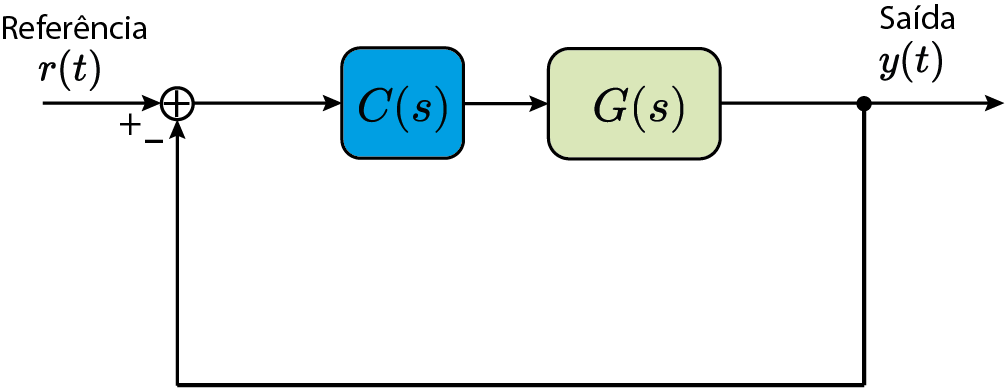
\includegraphics[width=0.62\linewidth]{malha_fechada_controle_s.png}
    \caption[Malha fechada no plano $s$]{Sistema de controle em malha fechada
    com realimentação unitária. O sinal de referência é comparado à saída,
    gerando o erro que alimenta o controlador $C(s)$; este atua sobre a planta
    $G(s)$.}
    \label{fig:malha_s}
\end{figure}

\begin{proposicao}[Função de transferência de malha fechada]
\label{prop:mf}
Para o sistema da Figura~\ref{fig:malha_s} com realimentação unitária, a função
de transferência da referência para a saída é
\begin{equation}
    G_f(s)=\frac{C(s)G(s)}{1+C(s)G(s)}.
    \label{eq:Gf_s}
\end{equation}
\end{proposicao}

\begin{proof}
Seja $E(s)=R(s)-Y(s)$ o erro. A saída é $Y(s)=C(s)G(s)E(s)=C(s)G(s)\left[R(s)-Y(s)\right]$.
Reagrupando, $\left[1+C(s)G(s)\right]Y(s)=C(s)G(s)R(s)$, de onde segue
imediatamente a Equação~\eqref{eq:Gf_s}.
\end{proof}

A dinâmica de $G_f(s)$ é, em geral, de ordem elevada. Contudo, o comportamento
transitório de muitos sistemas é bem aproximado por um par de \emph{polos
dominantes} de segunda ordem --- os polos de malha fechada mais próximos do eixo
imaginário, que decaem mais lentamente e, portanto, ditam a resposta. Isso
justifica estudar em detalhe o protótipo de segunda ordem.

\begin{definicao}[Sistema de segunda ordem padrão]
\label{def:2ordem}
Um sistema de segunda ordem \emph{padrão} (subamortecido, sem zeros) tem função
de transferência de malha fechada
\begin{equation}
    G_f(s)=\frac{\wn^2}{s^2+2\xi\wn s+\wn^2},
    \label{eq:2ordem}
\end{equation}
em que $\wn>0$ é a \textbf{frequência natural não amortecida} e
$0\le\xi<1$ é o \textbf{coeficiente de amortecimento}.
\end{definicao}

Observe que $G_f(0)=1$: em regime permanente, a saída acompanha um degrau
unitário sem erro, o que torna esse protótipo conveniente para definir os
critérios transitórios.

\subsection{Polos dominantes de segunda ordem}

\begin{proposicao}[Polos do protótipo de segunda ordem]
\label{prop:polos}
Para $0\le\xi<1$, os polos de \eqref{eq:2ordem} são o par complexo conjugado
\begin{equation}
    s_{1,2}=-\xi\wn\pm j\,\wn\sqrt{1-\xi^2}.
    \label{eq:polos_s}
\end{equation}
\end{proposicao}

\begin{proof}
Os polos são as raízes do denominador $s^2+2\xi\wn s+\wn^2=0$. Pela fórmula de
Bhaskara,
\[
s=\frac{-2\xi\wn\pm\sqrt{4\xi^2\wn^2-4\wn^2}}{2}
 =-\xi\wn\pm\wn\sqrt{\xi^2-1}.
\]
Como $0\le\xi<1$, tem-se $\xi^2-1<0$ e $\sqrt{\xi^2-1}=j\sqrt{1-\xi^2}$, o que
fornece \eqref{eq:polos_s}.
\end{proof}

É conveniente definir a parte real e a parte imaginária dos polos:
\begin{equation}
    \sd \triangleq \xi\wn \quad(\text{fator de decaimento}),\qquad
    \wda \triangleq \wn\sqrt{1-\xi^2}\quad(\text{frequência amortecida}).
    \label{eq:sd_wd}
\end{equation}
Assim, $s_{1,2}=-\sd\pm j\wda$. A Figura~\ref{fig:polos_xiwn} mostra a
interpretação geométrica desses parâmetros no plano $s$.

\begin{figure}[H]
    \centering
    
\includegraphics[width=0.62\linewidth]{polos_dominantes_xi_wn.png}
    \caption[Geometria dos polos no plano $s$]{Localização dos polos dominantes
    no plano $s$. A distância do polo à origem é a frequência natural $\wn$; o
    ângulo $\theta$ com o eixo imaginário satisfaz $\cos\theta=\xi$ (aqui medido
    de modo que $\sin\theta=\sqrt{1-\xi^2}$). Aumentar $\wn$ afasta os polos da
    origem (resposta mais rápida); aumentar $\xi$ aproxima-os do eixo real
    (resposta mais amortecida).}
    \label{fig:polos_xiwn}
\end{figure}

\begin{figure}[H]
    \centering
    
\includegraphics[width=0.45\linewidth]{polos_dominantes.png}
    \caption[Par de polos complexos conjugados]{Par de polos complexos
    conjugados $s_{1,2}=-\sd\pm j\wda$ para o caso subamortecido
    ($0\le\xi<1$). A parte real $-\sd$ governa o decaimento exponencial da
    envoltória; a parte imaginária $\pm\wda$ governa a frequência de oscilação.}
    \label{fig:polos}
\end{figure}

\subsection{Resposta ao degrau unitário}

Aplica-se ao sistema \eqref{eq:2ordem} um degrau unitário $U(s)=1/s$. A saída no
domínio de Laplace é
\begin{equation}
    Y(s)=G_f(s)U(s)=\frac{\wn^2}{\left(s^2+2\xi\wn s+\wn^2\right)s}.
    \label{eq:Ys}
\end{equation}
A resposta temporal é obtida pela transformada inversa de Laplace,
$y(t)=\Ltr^{-1}\{Y(s)\}$. O resultado é o Teorema~\ref{teo:resposta_degrau}.

\begin{teorema}[Resposta ao degrau do sistema de segunda ordem]
\label{teo:resposta_degrau}
A resposta do sistema \eqref{eq:2ordem} ao degrau unitário, para $0\le\xi<1$ e
$t\ge 0$, é
\begin{equation}
    y(t)=1-\frac{e^{-\sd t}}{\sqrt{1-\xi^2}}
        \sin\!\left(\wda t+\phi\right),
    \qquad \phi=\arctan\!\left(\frac{\sqrt{1-\xi^2}}{\xi}\right)=\arccos\xi,
    \label{eq:yt}
\end{equation}
com $\sd$ e $\wda$ dados por \eqref{eq:sd_wd}.
\end{teorema}

\begin{proof}
Faz-se a expansão em frações parciais de \eqref{eq:Ys}:
\[
Y(s)=\frac{\wn^2}{s\left(s^2+2\xi\wn s+\wn^2\right)}
    =\frac{A}{s}+\frac{Bs+C}{s^2+2\xi\wn s+\wn^2}.
\]
Multiplicando por $s$ e fazendo $s\to 0$ obtém-se $A=1$. Igualando os numeradores,
\[
\wn^2=A\left(s^2+2\xi\wn s+\wn^2\right)+(Bs+C)s.
\]
Comparando o coeficiente de $s^2$: $0=A+B\Rightarrow B=-1$. Comparando o de $s^1$:
$0=2A\xi\wn+C\Rightarrow C=-2\xi\wn$. Logo,
\[
Y(s)=\frac{1}{s}-\frac{s+2\xi\wn}{s^2+2\xi\wn s+\wn^2}.
\]
Completa-se o quadrado no denominador: $s^2+2\xi\wn s+\wn^2=(s+\sd)^2+\wda^2$,
com $\sd=\xi\wn$ e $\wda=\wn\sqrt{1-\xi^2}$. Reescreve-se o numerador de modo a
identificar as transformadas de seno e cosseno amortecidos:
\[
s+2\xi\wn=(s+\sd)+\xi\wn=(s+\sd)+\frac{\sd}{\wda}\,\wda .
\]
Portanto,
\[
Y(s)=\frac{1}{s}
     -\frac{s+\sd}{(s+\sd)^2+\wda^2}
     -\frac{\sd}{\wda}\cdot\frac{\wda}{(s+\sd)^2+\wda^2}.
\]
Usando os pares $\Ltr^{-1}\!\left\{\tfrac{s+\sd}{(s+\sd)^2+\wda^2}\right\}
=e^{-\sd t}\cos\wda t$ e
$\Ltr^{-1}\!\left\{\tfrac{\wda}{(s+\sd)^2+\wda^2}\right\}=e^{-\sd t}\sin\wda t$,
\[
y(t)=1-e^{-\sd t}\left(\cos\wda t+\frac{\sd}{\wda}\sin\wda t\right).
\]
Resta compactar a combinação linear de seno e cosseno. Com
$\sd/\wda=\xi/\sqrt{1-\xi^2}$,
\[
\cos\wda t+\frac{\xi}{\sqrt{1-\xi^2}}\sin\wda t
=\frac{1}{\sqrt{1-\xi^2}}\left(\sqrt{1-\xi^2}\cos\wda t+\xi\sin\wda t\right)
=\frac{1}{\sqrt{1-\xi^2}}\sin(\wda t+\phi),
\]
em que $\phi$ satisfaz $\cos\phi=\xi$ e $\sin\phi=\sqrt{1-\xi^2}$, isto é,
$\phi=\arctan\!\big(\sqrt{1-\xi^2}/\xi\big)=\arccos\xi$. Substituindo, obtém-se
\eqref{eq:yt}.
\end{proof}

\begin{observacao}
A Equação~\eqref{eq:yt} tem estrutura muito informativa: é o valor final
($=1$) subtraído de uma senoide de frequência $\wda$ cuja amplitude decai como
$e^{-\sd t}$. O fator $\sd=\xi\wn$ controla a \emph{velocidade de decaimento} e
$\wda$ controla a \emph{frequência das oscilações}. Todos os critérios
transitórios a seguir são consequências diretas dessa expressão.
\end{observacao}

\subsection{Tempo de subida $t_r$}

\begin{definicao}[Tempo de subida]
O \textbf{tempo de subida} $t_r$ de um sistema subamortecido é o instante em que
a resposta ao degrau atinge, pela primeira vez, o valor final, isto é, $y(t_r)=1$.
\end{definicao}

\begin{figure}[H]
    \centering
    
\includegraphics[width=0.62\linewidth]{resposta_2ordem_tr.png}
    \caption[Tempo de subida]{Definição do tempo de subida $t_r$: primeiro
    instante em que a resposta cruza o valor final unitário. Para sistemas
    subamortecidos adota-se o cruzamento de $0\%$ a $100\%$.}
    \label{fig:tr}
\end{figure}

\begin{proposicao}[Expressão do tempo de subida]
\label{prop:tr}
Para o sistema \eqref{eq:2ordem} com $0\le\xi<1$,
\begin{equation}
    t_r=\frac{\pi-\phi}{\wda}=\frac{1}{\wda}\arctantwo(\wda,-\sd),
    \qquad \phi=\arccos\xi.
    \label{eq:tr}
\end{equation}
\end{proposicao}

\begin{proof}
Impondo $y(t_r)=1$ em \eqref{eq:yt},
\[
1=1-\frac{e^{-\sd t_r}}{\sqrt{1-\xi^2}}\sin(\wda t_r+\phi)
\;\Longrightarrow\;
\frac{e^{-\sd t_r}}{\sqrt{1-\xi^2}}\sin(\wda t_r+\phi)=0.
\]
Como $e^{-\sd t_r}\neq 0$, é necessário que $\sin(\wda t_r+\phi)=0$, ou seja,
$\wda t_r+\phi=n\pi$ para $n\in\mathbb{Z}$. O primeiro cruzamento com o valor final
(o menor $t_r>0$) corresponde a $n=1$, portanto $\wda t_r+\phi=\pi$, de onde
$t_r=(\pi-\phi)/\wda$.

Para a forma compacta, note que $\phi=\arccos\xi$ é o ângulo do vetor
$(\sd,\wda)$ (pois $\cos\phi=\xi=\sd/\wn$ e $\sin\phi=\wda/\wn$). O suplemento
$\pi-\phi$ é justamente o argumento do polo $s_1=-\sd+j\wda$, que se encontra no
segundo quadrante:
\[
\pi-\phi=\arctantwo(\wda,-\sd).
\]
Substituindo, obtém-se \eqref{eq:tr}.
\end{proof}

\begin{observacao}
A Proposição~\ref{prop:tr} mostra que $t_r$ é inversamente proporcional a $\wda$:
polos mais afastados do eixo real (maior $\wda$) produzem respostas mais rápidas.
O ângulo $\pi-\phi$ é exatamente o argumento do polo dominante no plano $s$ ---
uma leitura puramente geométrica do tempo de subida.
\end{observacao}

\subsection{Tempo de pico $t_p$}

\begin{definicao}[Tempo de pico]
O \textbf{tempo de pico} $t_p$ é o instante em que a resposta ao degrau atinge
seu valor máximo, caracterizado pela condição estacionária
$\left.\dfrac{dy}{dt}\right|_{t=t_p}=0$.
\end{definicao}

\begin{figure}[H]
    \centering
    
\includegraphics[width=0.62\linewidth]{resposta_2ordem_tp.png}
    \caption[Tempo de pico]{Definição do tempo de pico $t_p$: instante do máximo
    da resposta, no qual a derivada temporal se anula.}
    \label{fig:tp}
\end{figure}

\begin{proposicao}[Expressão do tempo de pico]
\label{prop:tp}
Para o sistema \eqref{eq:2ordem} com $0\le\xi<1$,
\begin{equation}
    t_p=\frac{\pi}{\wda}.
    \label{eq:tp}
\end{equation}
\end{proposicao}

\begin{proof}
Deriva-se \eqref{eq:yt}. Aplicando a regra do produto ao termo
$e^{-\sd t}\sin(\wda t+\phi)$,
\[
\frac{dy}{dt}
=\frac{e^{-\sd t}}{\sqrt{1-\xi^2}}
   \Big[\sd\sin(\wda t+\phi)-\wda\cos(\wda t+\phi)\Big].
\]
A combinação entre colchetes é da forma $A\sin\alpha-B\cos\alpha$ com
$A=\sd$ e $B=\wda$, que se reescreve como $R\sin(\alpha-\psi)$ com
$R=\sqrt{\sd^2+\wda^2}=\wn$ e $\tan\psi=B/A=\wda/\sd=\tan\phi$, logo $\psi=\phi$.
Portanto,
\[
\frac{dy}{dt}
=\frac{\wn\,e^{-\sd t}}{\sqrt{1-\xi^2}}\sin\big((\wda t+\phi)-\phi\big)
=\frac{\wn\,e^{-\sd t}}{\sqrt{1-\xi^2}}\sin(\wda t).
\]
Impondo $dy/dt=0$ e descartando o fator exponencial, resta $\sin(\wda t_p)=0$,
isto é, $\wda t_p=n\pi$. O primeiro máximo ($n=1$) ocorre em $t_p=\pi/\wda$.
\end{proof}

\subsection{Sobressinal $M_p$}

\begin{definicao}[Sobressinal máximo]
O \textbf{sobressinal máximo} é o excesso da resposta sobre o valor final,
avaliado no instante de pico:
\begin{equation}
    M_p=y(t_p)-y(\infty)=y(t_p)-1.
    \label{eq:Mp_def}
\end{equation}
Frequentemente é expresso em forma percentual, $M_p\%=100\,M_p$.
\end{definicao}

\begin{figure}[H]
    \centering
    
\includegraphics[width=0.62\linewidth]{resposta_2ordem_Mp.png}
    \caption[Sobressinal]{Definição do sobressinal $M_p$: diferença entre o valor
    de pico e o valor final da resposta ao degrau.}
    \label{fig:Mp}
\end{figure}

\begin{teorema}[Sobressinal em função do amortecimento]
\label{teo:Mp}
Para o sistema \eqref{eq:2ordem} com $0\le\xi<1$,
\begin{equation}
    M_p=\exp\!\left(-\frac{\pi\,\xi}{\sqrt{1-\xi^2}}\right).
    \label{eq:Mp}
\end{equation}
\end{teorema}

\begin{proof}
Substitui-se $t_p=\pi/\wda$ (Proposição~\ref{prop:tp}) em \eqref{eq:yt}:
\[
y(t_p)=1-\frac{e^{-\sd \pi/\wda}}{\sqrt{1-\xi^2}}\sin(\pi+\phi).
\]
Como $\sin(\pi+\phi)=-\sin\phi=-\sqrt{1-\xi^2}$,
\[
y(t_p)=1-\frac{e^{-\sd\pi/\wda}}{\sqrt{1-\xi^2}}\big(-\sqrt{1-\xi^2}\big)
      =1+e^{-\sd\pi/\wda}.
\]
Logo, por \eqref{eq:Mp_def}, $M_p=e^{-\sd\pi/\wda}$. Finalmente, usando
$\dfrac{\sd}{\wda}=\dfrac{\xi\wn}{\wn\sqrt{1-\xi^2}}=\dfrac{\xi}{\sqrt{1-\xi^2}}$,
obtém-se \eqref{eq:Mp}.
\end{proof}

Em projeto, o requisito é tipicamente dado como um limite de sobressinal (por
exemplo $M_p\le 10\%$) e precisamos do amortecimento $\xi$ correspondente. Ou
seja, é preciso \emph{inverter} a relação \eqref{eq:Mp}.

\begin{corolario}[Amortecimento em função do sobressinal]
\label{cor:xi}
Invertendo \eqref{eq:Mp}, o coeficiente de amortecimento que produz um
sobressinal $M_p$ é
\begin{equation}
    \xi=\left|\frac{\ln M_p}{\sqrt{\pi^2+\ln^2 M_p}}\right|.
    \label{eq:xi}
\end{equation}
\end{corolario}

\begin{proof}
Aplica-se o logaritmo natural a \eqref{eq:Mp}:
\[
\ln M_p=-\frac{\pi\,\xi}{\sqrt{1-\xi^2}}
\;\Longrightarrow\;
\sqrt{1-\xi^2}=-\frac{\pi\,\xi}{\ln M_p}.
\]
Elevando ao quadrado,
\[
1-\xi^2=\frac{\pi^2\xi^2}{\ln^2 M_p}
\;\Longrightarrow\;
\ln^2 M_p-\xi^2\ln^2 M_p=\pi^2\xi^2
\;\Longrightarrow\;
\ln^2 M_p=\big(\pi^2+\ln^2 M_p\big)\xi^2.
\]
Isolando $\xi^2$ e extraindo a raiz (com $0\le\xi<1$),
\[
\xi^2=\frac{\ln^2 M_p}{\pi^2+\ln^2 M_p}
\;\Longrightarrow\;
\xi=\left|\frac{\ln M_p}{\sqrt{\pi^2+\ln^2 M_p}}\right|,
\]
que é \eqref{eq:xi}. O valor absoluto assegura $\xi\ge 0$, já que $\ln M_p<0$
para $0<M_p<1$.
\end{proof}

\subsection{Envelope da resposta e boa prática de projeto}

A amplitude das oscilações em \eqref{eq:yt} está limitada pela envoltória
$\pm\,e^{-\sd t}/\sqrt{1-\xi^2}$. A Figura~\ref{fig:env} ilustra como o
amortecimento define a forma da resposta.

\begin{figure}[H]
    \centering
    
\includegraphics[width=0.62\linewidth]{enveloped_xi.png}
    \caption[Envelope de sobressinal]{Resposta ao degrau com
    $0{,}4\le\xi\le 0{,}8$ e sua envoltória exponencial. Nessa faixa obtém-se um
    compromisso adequado entre rapidez e sobressinal moderado.}
    \label{fig:env}
\end{figure}

\begin{destaque}
\textbf{Boa prática de projeto.} Recomenda-se, em geral,
\[
0{,}4\le\xi\le 0{,}8.
\]
\begin{itemize}[nosep]
    \item $\xi<0{,}4$: sobressinal elevado (transitório muito oscilatório);
    \item $\xi>0{,}8$: resposta demasiadamente lenta (transitório
    sobreamortecido).
\end{itemize}
\end{destaque}

\subsection{Tempo de acomodação $t_s$}

\begin{definicao}[Tempo de acomodação]
O \textbf{tempo de acomodação} $t_s$ é o menor instante a partir do qual a
resposta permanece dentro de uma faixa de tolerância $\pm\epsilon$ em torno do
valor final:
\[
t_s:\ \forall\, t\ge t_s \Rightarrow |y(t)-y(\infty)|\le\epsilon.
\]
\end{definicao}

\begin{figure}[H]
    \centering
    
\includegraphics[width=0.62\linewidth]{resposta_2ordem_ts.png}
    \caption[Tempo de acomodação]{Definição do tempo de acomodação $t_s$: a
    resposta entra e permanece na faixa de tolerância $\pm\epsilon$
    (tipicamente $2\%$ ou $5\%$) determinada pela envoltória exponencial.}
    \label{fig:ts}
\end{figure}

\begin{proposicao}[Expressão do tempo de acomodação]
\label{prop:ts}
Aproximando a fronteira da faixa de tolerância pela envoltória exponencial,
$e^{-\sd t_s}\le\epsilon$, o tempo de acomodação é
\begin{equation}
    t_s=-\frac{\ln\epsilon}{\sd}=-\frac{\ln\epsilon}{\xi\wn}.
    \label{eq:ts_geral}
\end{equation}
Em particular:
\begin{align}
    \text{Tolerância de } 5\%\ (\epsilon=0{,}05):&\quad
    t_s=-\frac{\ln 0{,}05}{\xi\wn}\approx\frac{3}{\xi\wn};
    \label{eq:ts5}\\[2pt]
    \text{Tolerância de } 2\%\ (\epsilon=0{,}02):&\quad
    t_s=-\frac{\ln 0{,}02}{\xi\wn}\approx\frac{4}{\xi\wn}.
    \label{eq:ts2}
\end{align}
\end{proposicao}

\begin{proof}
O desvio $|y(t)-1|$ é dominado pela envoltória $e^{-\sd t}/\sqrt{1-\xi^2}$.
Adotando o critério prático $e^{-\sd t_s}=\epsilon$ (o fator
$1/\sqrt{1-\xi^2}$ é omitido nessa aproximação usual), aplica-se o logaritmo:
$-\sd t_s=\ln\epsilon$, logo $t_s=-\ln\epsilon/\sd$, com $\sd=\xi\wn$. Para os
valores numéricos, $-\ln 0{,}05=2{,}996\approx 3$ e $-\ln 0{,}02=3{,}912\approx 4$,
o que produz \eqref{eq:ts5} e \eqref{eq:ts2}.
\end{proof}

\begin{observacao}
As Proposições~\ref{prop:tr}--\ref{prop:ts} revelam a divisão de papéis entre os
dois parâmetros do sistema de segunda ordem: $\wda$ (e, portanto, $\wn$) governa a
\emph{velocidade} ($t_r$ e $t_p$), enquanto o produto $\sd=\xi\wn$ governa o
\emph{amortecimento} ($t_s$) e $\xi$ isoladamente governa o \emph{sobressinal}
($M_p$). Especificar $M_p$ e $t_s$ equivale, portanto, a especificar $\xi$ e
$\wn$ --- e, por consequência, a posição desejada dos polos dominantes.
\end{observacao}

\section{Erros em regime estacionário}
\label{sec:erros}

Concluída a análise transitória, passamos ao regime permanente. A pergunta é:
depois que o transitório se extingue, quão próxima a saída fica da referência? A
resposta depende de duas coisas: o \emph{tipo} da entrada e o \emph{tipo} do
sistema.

\subsection{Tipo do sistema}

\begin{definicao}[Tipo do sistema --- plano $s$]
\label{def:tipo_s}
Seja a função de transferência de malha aberta escrita na forma
\begin{equation}
    G(s)=\frac{K\,(T_a s+1)(T_b s+1)\cdots(T_m s+1)}
              {s^N\,(T_1 s+1)(T_2 s+1)\cdots(T_p s+1)}.
    \label{eq:tipo_s}
\end{equation}
O \textbf{tipo} do sistema é o número $N$ de polos na origem: tipo $0$ se $N=0$,
tipo $1$ se $N=1$, tipo $2$ se $N=2$, e assim por diante.
\end{definicao}

\begin{destaque}
O número de polos na origem ($s=0$), ou equivalentemente o número de
\emph{integradores} presentes na malha, define o tipo do sistema. Como veremos,
cada integrador acrescenta uma ``ordem'' de capacidade de anular erros.
\end{destaque}

As Figuras~\ref{fig:tipo0}--\ref{fig:tipo2} ilustram o comportamento de sistemas
de tipos crescentes diante de entradas de referência de degrau, rampa e parábola.

\begin{figure}[H]
    \centering
    
\includegraphics[width=0.55\linewidth]{tipo0_degrau.png}
    \caption[Sistema tipo 0 --- degrau]{Sistema tipo 0,
    $G(s)=\dfrac{2s+1}{s^2+s+1}$, resposta ao degrau. Sem integrador, o sistema
    apresenta \emph{erro de posição não nulo}: a saída estabiliza abaixo da
    referência.}
    \label{fig:tipo0}
\end{figure}

\begin{figure}[H]
    \centering
    \begin{subfigure}{0.48\linewidth}
        \centering
        
\includegraphics[width=\linewidth]{tipo1_degrau.png}
        \caption{Resposta ao degrau: erro nulo.}
    \end{subfigure}\hfill
    \begin{subfigure}{0.48\linewidth}
        \centering
        
\includegraphics[width=\linewidth]{tipo1_rampa.png}
        \caption{Resposta à rampa: erro finito constante.}
    \end{subfigure}
    \caption[Sistema tipo 1]{Sistema tipo 1,
    $G(s)=\dfrac{2s+1}{s(s^2+s+1)}$. O integrador anula o erro ao degrau, mas
    resta um erro finito de velocidade quando a entrada é uma rampa.}
    \label{fig:tipo1}
\end{figure}

\begin{figure}[H]
    \centering
    \begin{subfigure}{0.32\linewidth}
        \centering
        
\includegraphics[width=\linewidth]{tipo2_degrau.png}
        \caption{Degrau.}
    \end{subfigure}\hfill
    \begin{subfigure}{0.32\linewidth}
        \centering
        
\includegraphics[width=\linewidth]{tipo2_rampa.png}
        \caption{Rampa.}
    \end{subfigure}\hfill
    \begin{subfigure}{0.32\linewidth}
        \centering
        
\includegraphics[width=\linewidth]{tipo2_parabola.png}
        \caption{Parábola.}
    \end{subfigure}
    \caption[Sistema tipo 2]{Sistema tipo 2,
    $G(s)=\dfrac{2s+1}{s^2(s^2+s+5)}$. Com dois integradores, o erro é nulo para
    degrau e rampa, restando um erro finito de aceleração para a entrada em
    parábola.}
    \label{fig:tipo2}
\end{figure}

A mesma ideia se aplica ao tempo discreto, com os polos na origem ($s=0$) do
plano $s$ correspondendo a polos em $z=1$ do plano $z$ --- afinal, $z=e^{sT}$
leva $s=0$ em $z=1$.

\begin{definicao}[Tipo do sistema --- plano $z$]
\label{def:tipo_z}
Seja a função de transferência de malha aberta discreta escrita como
\begin{equation}
    G(z)=\frac{1}{(z-1)^N}\,\frac{N(z)}{D(z)},
    \label{eq:tipo_z}
\end{equation}
com $N(1)\neq 0$ e $D(1)\neq 0$. O \textbf{tipo} do sistema discreto é o número
$N$ de polos em $z=1$.
\end{definicao}

\begin{destaque}
\textbf{Consequência prática (malha fechada).}
\begin{itemize}[nosep]
    \item Tipo 1: erro nulo para entrada em \emph{degrau};
    \item Tipo 2: erro nulo para entrada em \emph{degrau} e \emph{rampa};
    \item Tipo 3: erro nulo para entrada em \emph{degrau}, \emph{rampa} e
    \emph{parábola}.
\end{itemize}
\end{destaque}

\subsection{Erro em regime estacionário no plano \texorpdfstring{$z$}{z}}

\begin{definicao}[Erro de rastreamento]
Para um sistema discreto em malha fechada com realimentação unitária
(Figura~\ref{fig:malha_erro}), o \textbf{erro de rastreamento} no instante $k$ é
\begin{equation}
    e[k]=r[k]-y[k].
\end{equation}
\end{definicao}

\begin{figure}[H]
    \centering
    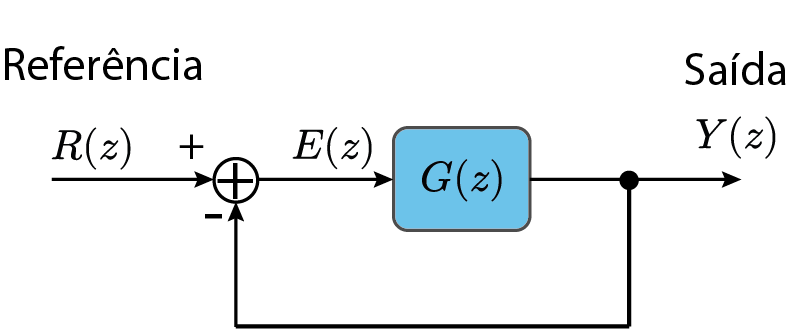
\includegraphics[width=0.6\linewidth]{malha_controle_erro.png}
    \caption[Malha de controle discreta e o erro]{Malha de controle discreta com
    realimentação unitária. O erro $E(z)=R(z)-Y(z)$ é a entrada do ramo direto de
    ganho $G(z)$, de modo que $Y(z)=G(z)E(z)$.}
    \label{fig:malha_erro}
\end{figure}

O cálculo do erro de regime baseia-se no teorema do valor final para a
transformada $\Ztr$.

\begin{teorema}[Teorema do valor final --- tempo discreto]
\label{teo:vf}
Se a sequência $e[k]$ converge quando $k\to\infty$ (equivalentemente, se
$(z-1)E(z)$ é analítica sobre e fora do círculo unitário), então
\begin{equation}
    \lim_{k\to\infty}e[k]=\lim_{z\to 1}(z-1)E(z).
    \label{eq:vf}
\end{equation}
\end{teorema}

\begin{proposicao}[Erro de malha fechada em função de $G(z)$]
\label{prop:Ez}
Para a malha da Figura~\ref{fig:malha_erro},
\begin{equation}
    E(z)=\frac{1}{1+G(z)}\,R(z),
    \label{eq:Ez}
\end{equation}
e, portanto, o erro em regime estacionário é
\begin{equation}
    e_{ss}=\lim_{z\to 1}(z-1)\,\frac{1}{1+G(z)}\,R(z).
    \label{eq:ess}
\end{equation}
\end{proposicao}

\begin{proof}
Da malha, $Y(z)=G(z)E(z)$ e $E(z)=R(z)-Y(z)$. Substituindo a primeira na
segunda, $E(z)=R(z)-G(z)E(z)$, ou seja, $\big(1+G(z)\big)E(z)=R(z)$, o que
fornece \eqref{eq:Ez}. Aplicando o Teorema~\ref{teo:vf} a $E(z)$ obtém-se
\eqref{eq:ess}.
\end{proof}

A seguir aplicamos \eqref{eq:ess} a cada tipo de entrada, definindo as
\emph{constantes de erro estático}.

\subsubsection{Erro de posição (entrada em degrau)}

A entrada em degrau tem transformada $R(z)=\dfrac{z}{z-1}$.

\begin{proposicao}[Constante de posição]
\label{prop:Kp}
Para um sistema tipo 0, $G(z)=N(z)/D(z)$ com $D(1)\neq 0$, o erro de posição é
\begin{equation}
    e_{ss}=\frac{1}{1+K_p},\qquad
    K_p\triangleq\lim_{z\to 1}G(z).
    \label{eq:Kp}
\end{equation}
\end{proposicao}

\begin{proof}
Substituindo $R(z)=z/(z-1)$ e $G(z)=N(z)/D(z)$ em \eqref{eq:ess},
\[
e_{ss}=\lim_{z\to 1}(z-1)\,\frac{1}{1+\frac{N(z)}{D(z)}}\,\frac{z}{z-1}
      =\lim_{z\to 1}\frac{z}{1+\frac{N(z)}{D(z)}}.
\]
O fator $(z-1)$ cancela-se com o polo do degrau. Como o limite do numerador é
$1$ e o do denominador é $1+\lim_{z\to1}G(z)$,
\[
e_{ss}=\frac{\displaystyle\lim_{z\to1}z}{\displaystyle\lim_{z\to1}\big(1+\tfrac{N(z)}{D(z)}\big)}
      =\frac{1}{1+K_p},
\]
com $K_p=\lim_{z\to1}N(z)/D(z)=\lim_{z\to1}G(z)$.
\end{proof}

\begin{corolario}
Para um sistema tipo $\ge 1$, $K_p=\infty$ e, portanto, $e_{ss}=0$: o erro de
posição é nulo.
\end{corolario}

\begin{proof}
Se $G(z)=\dfrac{1}{z-1}\dfrac{N(z)}{D(z)}$ (tipo 1), então, por \eqref{eq:ess}
com $R(z)=z/(z-1)$,
\[
e_{ss}=\lim_{z\to1}(z-1)\frac{1}{1+\frac{1}{z-1}\frac{N(z)}{D(z)}}\frac{z}{z-1}
      =\lim_{z\to1}\frac{z(z-1)}{(z-1)+\frac{N(z)}{D(z)}}
      =\frac{0}{N(1)/D(1)}=0,
\]
pois o numerador tende a $0$ e o denominador a $N(1)/D(1)\neq 0$.
\end{proof}

\subsubsection{Erro de velocidade (entrada em rampa)}

A entrada em rampa tem transformada $R(z)=\dfrac{z}{(z-1)^2}$.

\begin{proposicao}[Constante de velocidade]
\label{prop:Kv}
Para um sistema tipo 1, $G(z)=\dfrac{1}{z-1}\dfrac{N(z)}{D(z)}$, o erro de
velocidade é
\begin{equation}
    e_{ss}=\frac{1}{K_v},\qquad
    K_v\triangleq\lim_{z\to 1}(z-1)G(z).
    \label{eq:Kv}
\end{equation}
\end{proposicao}

\begin{proof}
Com $R(z)=z/(z-1)^2$ em \eqref{eq:ess},
\[
e_{ss}=\lim_{z\to1}(z-1)\frac{1}{1+\frac{1}{z-1}\frac{N(z)}{D(z)}}\frac{z}{(z-1)^2}
      =\lim_{z\to1}\frac{\frac{z}{z-1}}{1+\frac{1}{z-1}\frac{N(z)}{D(z)}}.
\]
Multiplicando numerador e denominador por $(z-1)$,
\[
e_{ss}=\lim_{z\to1}\frac{z}{(z-1)+\frac{N(z)}{D(z)}}
      =\frac{1}{\lim_{z\to1}\frac{N(z)}{D(z)}}
      =\frac{1}{K_v},
\]
já que $(z-1)\to 0$. Aqui $K_v=\lim_{z\to1}N(z)/D(z)=\lim_{z\to1}(z-1)G(z)$.
\end{proof}

\begin{corolario}
Para um sistema tipo 0, $K_v=0$ e o erro de velocidade é infinito (a saída não
consegue seguir a rampa). Para um sistema tipo $\ge 2$, $K_v=\infty$ e o erro de
velocidade é nulo.
\end{corolario}

\begin{proof}[Esboço]
Para o tipo 2, $G(z)=\dfrac{1}{(z-1)^2}\dfrac{N(z)}{D(z)}$ e
\[
e_{ss}=\lim_{z\to1}\frac{\frac{z}{z-1}}{1+\frac{1}{(z-1)^2}\frac{N(z)}{D(z)}}
      =\lim_{z\to1}\frac{z(z-1)}{(z-1)^2+\frac{N(z)}{D(z)}}
      =\frac{0}{N(1)/D(1)}=0.
\]
\end{proof}

\subsubsection{Erro de aceleração (entrada em parábola)}

A entrada em parábola tem transformada $R(z)=\dfrac{z(z+1)}{(z-1)^3}$.

\begin{proposicao}[Constante de aceleração]
\label{prop:Ka}
Para um sistema tipo 2, o erro de aceleração é
\begin{equation}
    e_{ss}=\frac{1}{K_a},\qquad
    K_a\triangleq\lim_{z\to 1}(z-1)^2 G(z).
    \label{eq:Ka}
\end{equation}
\end{proposicao}

\begin{proof}[Esboço]
Substituindo $R(z)=z(z+1)/(z-1)^3$ em \eqref{eq:ess} e simplificando os fatores
$(z-1)$ de modo análogo às provas anteriores, o termo dominante do denominador é
$(z-1)^2 G(z)$, cujo limite define $K_a$; o numerador tende a
$\lim_{z\to1}z(z+1)/(z+1)=1$ após o cancelamento, resultando em $e_{ss}=1/K_a$.
\end{proof}

\subsection{Quadro resumo}

Reunindo as Proposições~\ref{prop:Kp}--\ref{prop:Ka}, obtém-se o quadro clássico
de erros em regime estacionário, organizado por tipo do sistema e por entrada.

\begin{table}[H]
    \centering
    \renewcommand{\arraystretch}{1.7}
    \begin{tabular}{>{\centering\arraybackslash}m{2.6cm}
                    >{\centering\arraybackslash}m{2.6cm}
                    >{\centering\arraybackslash}m{2.6cm}
                    >{\centering\arraybackslash}m{2.6cm}}
        \toprule
        \rowcolor{corbox}
        \textbf{Sistema} & \textbf{Degrau} & \textbf{Rampa} & \textbf{Parábola}\\
        \midrule
        Tipo 0 & $\dfrac{1}{1+K_p}$ & $\infty$ & $\infty$\\
        Tipo 1 & $0$ & $\dfrac{1}{K_v}$ & $\infty$\\
        Tipo 2 & $0$ & $0$ & $\dfrac{1}{K_a}$\\
        \bottomrule
    \end{tabular}
    \caption[Erros em regime estacionário]{Erro em regime estacionário
    $e_{ss}$ em função do tipo do sistema e da entrada de referência.}
    \label{tab:erros}
\end{table}

\begin{destaque}
As \textbf{constantes de erro estático} são
\begin{align*}
    K_p&=\lim_{z\to 1}G(z),\\
    K_v&=\lim_{z\to 1}(z-1)\,G(z),\\
    K_a&=\lim_{z\to 1}(z-1)^2\,G(z).
\end{align*}
Cada polo em $z=1$ (isto é, cada integrador) eleva o tipo do sistema em uma
unidade, anulando o erro para a entrada imediatamente inferior e tornando finito
o erro para a entrada correspondente.
\end{destaque}

\section{Estratégias de projeto}
\label{sec:estrategias}

Estabelecidos os critérios de desempenho, resta a questão prática: \emph{como}
obter o controlador digital $C(z)$? Existem duas grandes estratégias, que
diferem na ordem em que a discretização é realizada.

\subsection{Projeto por emulação}

Na \textbf{emulação}, projeta-se primeiro um controlador contínuo $C(s)$ ---
usando as ferramentas clássicas do plano $s$, como lugar geométrico das raízes
(LGR), diagrama de Bode e alocação de polos --- e só então esse controlador é
\emph{discretizado} (por Tustin, Euler \emph{backward}, etc.), gerando $C(z)$.

\begin{figure}[H]
    \centering
    
\includegraphics[width=0.85\linewidth]{projeto_c2d.png}
    \caption[Projeto por emulação]{Fluxo do projeto por emulação: o controlador é
    projetado no domínio contínuo ($s$) e depois convertido para o domínio
    discreto ($z$). A conversão ``$c2d$'' (\emph{continuous to discrete}) é a
    etapa de discretização do controlador.}
    \label{fig:c2d}
\end{figure}

\begin{destaque}
\textbf{Emulação --- vantagens e desvantagens.}

\emph{Vantagens:}
\begin{itemize}[nosep]
    \item projeto no domínio $s$ com ferramentas consagradas (LGR, Bode,
    alocação de polos).
\end{itemize}

\emph{Desvantagens:}
\begin{itemize}[nosep]
    \item despreza-se o efeito do segurador de ordem zero (ZOH);
    \item requer \textbf{discretização do controlador} (Tustin, Euler
    \emph{backward}, etc.);
    \item o desempenho em tempo discreto pode ser degradado;
    \item exige frequência de amostragem elevada para que a aproximação contínua
    seja válida.
\end{itemize}
\end{destaque}

\subsection{Projeto direto em \texorpdfstring{$z$}{z}}

No \textbf{projeto direto em $z$}, a ordem é invertida: discretiza-se primeiro a
\emph{planta} (incluindo o efeito do ZOH) e o controlador $C(z)$ é projetado
diretamente no plano $z$.

\begin{figure}[H]
    \centering
    
\includegraphics[width=0.45\linewidth]{projeto_path_d2d.png}
    \caption[Projeto direto em $z$]{Fluxo do projeto direto em $z$: a planta é
    discretizada e todo o projeto do controlador ocorre no domínio $z$.}
    \label{fig:d2d}
\end{figure}

\begin{destaque}
\textbf{Projeto direto em $z$ --- vantagens e desvantagens.}

\emph{Vantagens:}
\begin{itemize}[nosep]
    \item permite considerar os efeitos da amostragem e do ZOH;
    \item preserva o desempenho especificado para o sistema;
    \item admite taxas de amostragem menores.
\end{itemize}

\emph{Desvantagens:}
\begin{itemize}[nosep]
    \item requer a \textbf{discretização da planta} (por exemplo, degrau
    invariante, Tustin, Euler \emph{backward});
    \item os métodos (LGR, Bode, alocação de polos) precisam ser aplicados no
    domínio $z$, cuja geometria é menos intuitiva.
\end{itemize}
\end{destaque}

A Figura~\ref{fig:zoh} mostra a malha física a ser discretizada: um conversor
D/A com ZOH, a planta contínua $G(s)$ e um amostrador na saída. A discretização
por \emph{degrau invariante} substitui o conjunto ZOH + planta por uma única
função discreta $G(z)$, resultando na malha inteiramente discreta da
Figura~\ref{fig:zoh_z}.

\begin{figure}[H]
    \centering
    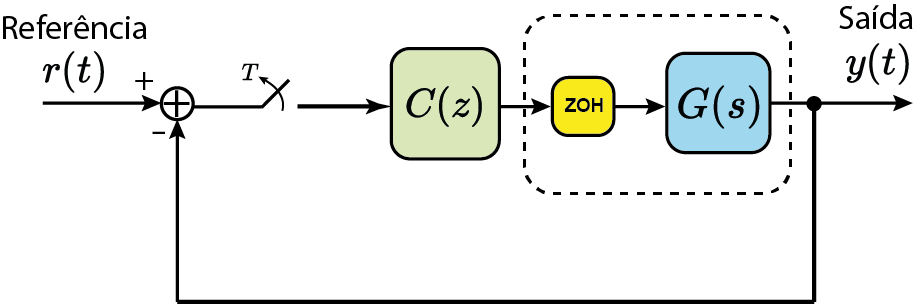
\includegraphics[width=0.9\linewidth]{malha_controle_zoh.png}
    \caption[Malha com ZOH]{Malha de controle digital com segurador de ordem
    zero (ZOH). O controlador discreto $C(z)$ gera amostras que são mantidas
    constantes pelo ZOH entre instantes de amostragem, atuando sobre a planta
    contínua $G(s)$. A discretização degrau-invariante do conjunto ZOH + planta
    fornece a equivalente discreta $G(z)$.}
    \label{fig:zoh}
\end{figure}

\begin{figure}[H]
    \centering
    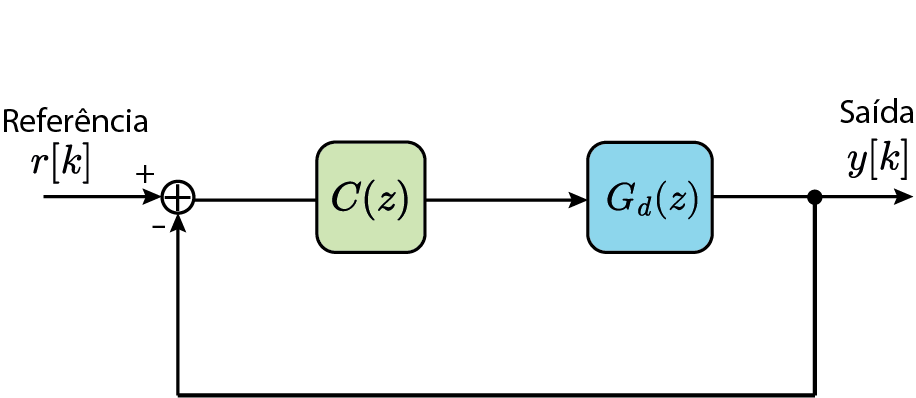
\includegraphics[width=0.9\linewidth]{malha_controle_zoh_planta_z.png}
    \caption[Malha totalmente discreta]{Após a discretização, obtém-se uma malha
    inteiramente em tempo discreto: controlador $C(z)$ e planta equivalente
    $G(z)$. Todo o projeto e a análise passam a ocorrer no plano $z$.}
    \label{fig:zoh_z}
\end{figure}

\section{Mapeamento de polos do plano \texorpdfstring{$s$}{s} para o plano \texorpdfstring{$z$}{z}}
\label{sec:mapeamento}

Para projetar diretamente em $z$, precisamos traduzir as especificações
transitórias --- expressas por meio de $\xi$ e $\wn$, isto é, por um par de
polos dominantes em $s$ --- para posições correspondentes no plano $z$. A ponte
é a relação fundamental $z=e^{sT}$, em que $T$ é o período de amostragem.

\begin{proposicao}[Imagem dos polos dominantes no plano $z$]
\label{prop:mapa}
Os polos dominantes $s_{1,2}=-\xi\wn\pm j\wn\sqrt{1-\xi^2}$ são mapeados, por
$z=e^{sT}$, no par
\begin{equation}
    z_{1,2}=e^{s_{1,2}T}=r\,e^{\pm j\theta},
    \qquad
    \begin{cases}
        r=e^{-T\xi\wn},\\[2pt]
        \theta=T\wn\sqrt{1-\xi^2}=T\wda.
    \end{cases}
    \label{eq:mapa}
\end{equation}
\end{proposicao}

\begin{proof}
Aplicando $z=e^{sT}$ a $s_{1,2}=-\xi\wn\pm j\wn\sqrt{1-\xi^2}$,
\[
z_{1,2}=e^{(-\xi\wn\pm j\wn\sqrt{1-\xi^2})T}
       =\underbrace{e^{-T\xi\wn}}_{r}\;
        \underbrace{e^{\pm jT\wn\sqrt{1-\xi^2}}}_{e^{\pm j\theta}}.
\]
Identificando módulo e argumento, $r=e^{-T\xi\wn}$ e
$\theta=T\wn\sqrt{1-\xi^2}=T\wda$.
\end{proof}

A Figura~\ref{fig:zgrid} mostra a grade de $\xi$ e $\wn$ constantes mapeada para
o interior do círculo unitário do plano $z$. Retas de $\xi$ constante tornam-se
\emph{espirais logarítmicas} e círculos de $\wn$ constante tornam-se curvas
fechadas em torno de $z=1$.

\begin{figure}[H]
    \centering
    \begin{subfigure}{0.52\linewidth}
        \centering
        
\includegraphics[width=\linewidth]{zgrid02.png}
        \caption{Curvas de $\xi$ constante.}
    \end{subfigure}\hfill
    \begin{subfigure}{0.45\linewidth}
        \centering
        
\includegraphics[width=\linewidth]{zgrid_wn.png}
        \caption{Curvas de $\wn$ constante.}
    \end{subfigure}
    \caption[Grade $\xi$--$\wn$ no plano $z$]{Mapeamento das curvas de
    amortecimento $\xi$ e frequência natural $\wn$ constantes para o plano $z$,
    obtido por $z=e^{sT}$. Essa ``$z$-grid'' permite ler graficamente onde os
    polos dominantes devem ser posicionados no plano $z$ para atender às
    especificações.}
    \label{fig:zgrid}
\end{figure}

\subsection{Exemplo numérico: dos requisitos aos polos em \texorpdfstring{$z$}{z}}

\begin{exemplo}[Localização dos polos desejados no plano $z$]
\label{ex:polos}
Especificam-se
\[
M_p\le 10\%,\qquad t_s\le 5\ \text{s}\ (\pm 2\%),\qquad T=0{,}1\ \text{s}.
\]
Determine o par de polos dominantes desejado no plano $z$.
\end{exemplo}

\noindent\textbf{Passo 1 --- amortecimento a partir do sobressinal.}
Do Corolário~\ref{cor:xi}, com $M_p=0{,}10$ e $\ln 0{,}10=-2{,}3026$:
\[
\xi=\left|\frac{\ln M_p}{\sqrt{\pi^2+\ln^2 M_p}}\right|
   =\frac{2{,}3026}{\sqrt{9{,}8696+5{,}3019}}
   =\frac{2{,}3026}{\sqrt{15{,}1715}}
   =\frac{2{,}3026}{3{,}8951}
   \approx 0{,}591.
\]

\noindent\textbf{Passo 2 --- frequência natural a partir do tempo de acomodação.}
Da Proposição~\ref{prop:ts}, critério de $2\%$ (Eq.~\eqref{eq:ts2}),
$t_s\approx 4/(\xi\wn)\le 5$, logo
\[
\xi\wn\ge\frac{4}{5}=0{,}8
\quad\Longrightarrow\quad
\wn\ge\frac{0{,}8}{0{,}591}\approx 1{,}354\ \text{rad/s}.
\]
Adotando a igualdade, $\wn=1{,}354$ rad/s. Assim,
\[
\sd=\xi\wn=0{,}8\ \text{s}^{-1},\qquad
\wda=\wn\sqrt{1-\xi^2}=1{,}354\sqrt{1-0{,}349}=1{,}354\times 0{,}807\approx 1{,}092\ \text{rad/s}.
\]
Os polos desejados no plano $s$ são $s_{1,2}=-0{,}8\pm j\,1{,}092$.

\noindent\textbf{Passo 3 --- mapeamento para o plano $z$.}
Da Proposição~\ref{prop:mapa} com $T=0{,}1$ s,
\[
r=e^{-T\xi\wn}=e^{-0{,}1\times 0{,}8}=e^{-0{,}08}\approx 0{,}9231,
\qquad
\theta=T\wda=0{,}1\times 1{,}092\approx 0{,}1092\ \text{rad}\ (\approx 6{,}26^\circ).
\]
Portanto,
\[
z_{1,2}=r\,e^{\pm j\theta}
       =0{,}9231\,(\cos 0{,}1092\pm j\sin 0{,}1092)
       \approx 0{,}9176\pm j\,0{,}1006.
\]

\begin{destaque}
\textbf{Resultado.} Os polos dominantes desejados no plano $z$ são
\[
z_{1,2}\approx 0{,}9176\pm j\,0{,}1006
\qquad(\,r\approx 0{,}923,\ \theta\approx 0{,}109\ \text{rad}\,).
\]
O projeto do controlador consistirá em posicionar os polos de malha fechada
nesses pontos.
\end{destaque}

\section{Estrutura do controlador e projeto analítico}
\label{sec:controlador}

\subsection{Compensadores de avanço e de atraso de fase}

Uma estrutura simples e amplamente utilizada é o compensador de primeira ordem,
com um polo e um zero reais.

\begin{definicao}[Compensador de avanço/atraso de fase]
\label{def:comp}
O compensador de avanço ou atraso de fase tem função de transferência
\begin{equation}
    C(z)=K\,\frac{z-a}{z-b},
    \label{eq:Cz}
\end{equation}
em que $K$ é o ganho, $a$ é o zero e $b$ é o polo do compensador.
\end{definicao}

\begin{destaque}
\textbf{Classificação (para polos e zeros reais no interior do círculo
unitário).}
\begin{itemize}[nosep]
    \item \textbf{Avanço de fase} (melhora o transitório):
    $-1<b<a<1$;
    \item \textbf{Atraso de fase} (melhora o regime permanente):
    $-1<a<b<1$.
\end{itemize}
\end{destaque}

\subsection{Malha fechada e formas de sintonia}

Com o compensador \eqref{eq:Cz} em série com a planta $G(z)$ e realimentação
unitária, a função de transferência de malha fechada é, por analogia à
Proposição~\ref{prop:mf},
\begin{empheq}[box=\tcbhighmath]{equation}
    G_f(z)=\frac{C(z)G(z)}{1+C(z)G(z)}.
    \label{eq:Gfz}
\end{empheq}

A escolha dos parâmetros $K$, $a$ e $b$ que fazem $G_f(z)$ atender às
especificações é chamada de \emph{sintonia} do compensador e pode ser feita por
diferentes métodos:
\begin{itemize}
    \item \textbf{forma analítica} (casamento direto de polos, detalhado a
    seguir);
    \item \textbf{lugar geométrico das raízes} (LGR);
    \item \textbf{resposta em frequência} (diagrama de Bode);
    \item \textbf{algoritmos de otimização} (algoritmos genéticos,
    \emph{particle swarm}, etc.).
\end{itemize}

\subsection{Projeto pela forma analítica}

A ideia do projeto analítico é impor que o \emph{denominador} de $G_f(z)$ seja
exatamente o polinômio cujas raízes são os polos dominantes desejados
$z_{1,2}=re^{\pm j\theta}$ obtidos na Seção~\ref{sec:mapeamento}.

\begin{proposicao}[Polinômio característico desejado]
\label{prop:carac}
Se a dinâmica de malha fechada deve ser de segunda ordem com polos
$z_{1,2}=e^{s_{1,2}T}=re^{\pm j\theta}$, então o polinômio característico
desejado é
\begin{equation}
    1+C(z)G(z)=z^2-(z_1+z_2)\,z+z_1 z_2
             =z^2-2r\cos\theta\,z+r^2.
    \label{eq:carac}
\end{equation}
\end{proposicao}

\begin{proof}
A equação característica da malha fechada \eqref{eq:Gfz} é
$1+C(z)G(z)=0$. Impondo que suas raízes sejam $z_1$ e $z_2$, o polinômio mônico
correspondente é
\[
(z-z_1)(z-z_2)=z^2-(z_1+z_2)z+z_1 z_2.
\]
Com $z_{1,2}=re^{\pm j\theta}$, a soma é
$z_1+z_2=r(e^{j\theta}+e^{-j\theta})=2r\cos\theta$ e o produto é
$z_1 z_2=r e^{j\theta}\cdot r e^{-j\theta}=r^2$, o que fornece \eqref{eq:carac}.
\end{proof}

\begin{observacao}[Procedimento de projeto analítico]
Reunindo os resultados, o projeto analítico de $C(z)=K\frac{z-a}{z-b}$ segue os
passos:
\begin{enumerate}[nosep]
    \item das especificações ($M_p$, $t_s$), obter $\xi$ e $\wn$
    (Corolário~\ref{cor:xi} e Proposição~\ref{prop:ts});
    \item mapear os polos para $z_{1,2}=re^{\pm j\theta}$
    (Proposição~\ref{prop:mapa}) e montar o polinômio desejado \eqref{eq:carac};
    \item impor $1+C(z)G(z)=z^2-2r\cos\theta\,z+r^2$ e igualar coeficientes,
    resolvendo para $K$, $a$ e $b$ (usando também condições de regime
    permanente, quando necessário, para fechar o sistema de equações).
\end{enumerate}
\end{observacao}

\section{Implementação digital do controlador}
\label{sec:implementacao}

Projetado $C(z)$, a última etapa é traduzi-lo em uma \emph{equação de
diferenças} executável em um microcontrolador. Considere o compensador
\eqref{eq:Cz} escrito como razão entre a transformada do sinal de controle
$U(z)$ e a do erro $E(z)$:
\begin{empheq}[box=\tcbhighmath]{equation}
    C(z)=K\,\frac{z-a}{z-b}=\frac{U(z)}{E(z)}.
    \label{eq:CzUE}
\end{empheq}

\begin{figure}[H]
    \centering
    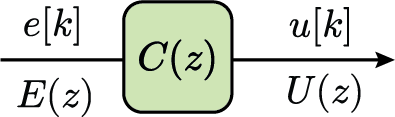
\includegraphics[width=0.45\linewidth]{discrete_control.png}
    \caption[Controlador discreto]{Controlador discreto: recebe o sinal de erro
    $e[k]$ e produz o sinal de controle $u[k]$. A relação entrada--saída é dada
    pela função de transferência $C(z)=U(z)/E(z)$.}
    \label{fig:discrete}
\end{figure}

\begin{proposicao}[Equação de diferenças do compensador]
\label{prop:diferencas}
O compensador \eqref{eq:CzUE} é realizado pela equação de diferenças recursiva
\begin{equation}
    u[k]=b\,u[k-1]+K\big(e[k]-a\,e[k-1]\big).
    \label{eq:diferencas}
\end{equation}
\end{proposicao}

\begin{proof}
Dividindo numerador e denominador de \eqref{eq:CzUE} por $z$, escreve-se o
compensador em potências de $z^{-1}$ (forma causal):
\[
C(z)=K\,\frac{1-a z^{-1}}{1-b z^{-1}}=\frac{U(z)}{E(z)}.
\]
Multiplicando em cruz,
\[
\big(1-b z^{-1}\big)U(z)=K\big(1-a z^{-1}\big)E(z),
\]
ou seja, $U(z)-b z^{-1}U(z)=K\,E(z)-Ka z^{-1}E(z)$. Aplicando a transformada
$\Ztr$ inversa e usando a propriedade do atraso, $z^{-1}X(z)\leftrightarrow x[k-1]$,
\[
u[k]-b\,u[k-1]=K\,e[k]-Ka\,e[k-1].
\]
Isolando $u[k]$ obtém-se \eqref{eq:diferencas}.
\end{proof}

\begin{observacao}
A Equação~\eqref{eq:diferencas} é \emph{recursiva} e \emph{causal}: o sinal de
controle atual $u[k]$ depende apenas de valores já conhecidos --- o controle
anterior $u[k-1]$, o erro atual $e[k]$ e o erro anterior $e[k-1]$. Isso a torna
diretamente implementável em software: bastam duas variáveis de memória (um
``$u$ anterior'' e um ``$e$ anterior'') atualizadas a cada iteração.
\end{observacao}

\subsection{Do algoritmo ao hardware}

A cada período de amostragem $T$, o microcontrolador lê a saída do sistema,
calcula o erro, avalia \eqref{eq:diferencas} e escreve o sinal de controle. Esse
laço é escrito em uma linguagem como C ou C++ e executado em plataformas como
Arduino, ESP32 ou Raspberry Pi (Figura~\ref{fig:hardware}).

\begin{figure}[H]
    \centering
    \begin{subfigure}{0.3\linewidth}
        \centering
        
\includegraphics[height=2.6cm,keepaspectratio]{arduino.png}
        \caption{Arduino.}
    \end{subfigure}\hfill
    \begin{subfigure}{0.3\linewidth}
        \centering
        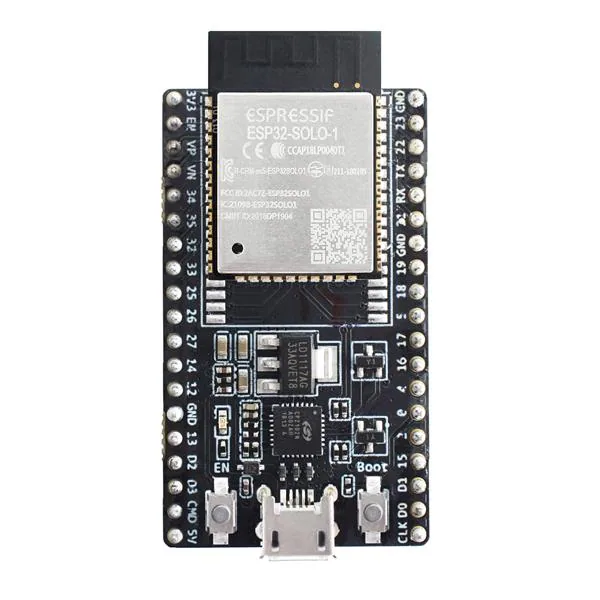
\includegraphics[height=2.6cm,keepaspectratio]{esp32.png}
        \caption{ESP32.}
    \end{subfigure}\hfill
    \begin{subfigure}{0.3\linewidth}
        \centering
        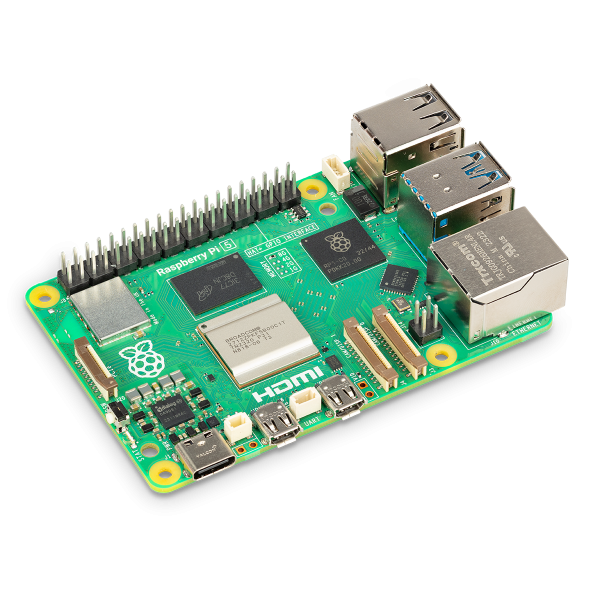
\includegraphics[height=2.6cm,keepaspectratio]{raspberrypi.png}
        \caption{Raspberry Pi.}
    \end{subfigure}
    \caption[Plataformas de implementação]{Plataformas típicas para
    implementação de controladores digitais. A equação de diferenças
    \eqref{eq:diferencas} é codificada e executada periodicamente nesses
    microcontroladores.}
    \label{fig:hardware}
\end{figure}

O trecho a seguir mostra um pseudocódigo de implementação em Arduino da
rotina executada a cada tique do temporizador (período $T$).

\begin{lstlisting}[style=arduino,caption={Pseudocódigo de implementação da equação de diferenças em Arduino.},captionpos=b]
void tick() {
    r = 1;                        // set-point (referencia)
    y = analogRead(input_pin);    // le a saida do sistema
    erro = r - y;                 // obtem o sinal de erro

    // sinal de controle: u[k] = b*u[k-1] + K*(e[k] - a*e[k-1])
    u = b*u_anterior + K*(erro - a*erro_anterior);

    erro_anterior = erro;         // atualiza erro p/ proxima iteracao
    u_anterior    = u;            // atualiza u    p/ proxima iteracao

    analogWrite(output_pin, u);   // atualiza a saida (atuador)
}
\end{lstlisting}

\begin{observacao}
Observe a correspondência direta entre a linha de cálculo do controle e a
Equação~\eqref{eq:diferencas}. As variáveis \texttt{u\_anterior} e
\texttt{erro\_anterior} implementam os atrasos $u[k-1]$ e $e[k-1]$. Em uma
implementação real deve-se ainda tratar a \emph{saturação} do atuador, a
\emph{escala} entre unidades de conversão A/D e D/A e a garantia de que a rotina
\texttt{tick()} seja chamada a intervalos regulares de período $T$.
\end{observacao}

\section*{Síntese do capítulo}
\addcontentsline{toc}{section}{Síntese do capítulo}

Este capítulo percorreu o caminho completo do projeto de controladores digitais.
Partimos da \emph{especificação} do desempenho em três famílias --- transitório,
regime permanente e robustez --- e deduzimos, a partir da resposta ao degrau do
sistema de segunda ordem padrão, as expressões fechadas do tempo de subida
\eqref{eq:tr}, tempo de pico \eqref{eq:tp}, sobressinal \eqref{eq:Mp} e tempo de
acomodação \eqref{eq:ts_geral}, além da inversão \eqref{eq:xi} que fornece o
amortecimento a partir do sobressinal desejado. Em seguida, caracterizamos o
\emph{erro em regime estacionário} pelo tipo do sistema, sintetizado na
Tabela~\ref{tab:erros} e nas constantes $K_p$, $K_v$ e $K_a$. Comparamos as duas
\emph{estratégias de projeto} --- emulação e projeto direto em $z$ --- e
mostramos, por meio do mapeamento $z=e^{sT}$, como transportar as especificações
para o plano $z$ (Exemplo~\ref{ex:polos}). Por fim, apresentamos a estrutura do
compensador de avanço/atraso, o \emph{projeto analítico} por casamento do
polinômio característico e a \emph{implementação digital} pela equação de
diferenças recursiva \eqref{eq:diferencas}, pronta para ser embarcada em um
microcontrolador.

\begin{figure}[H]
    \centering
    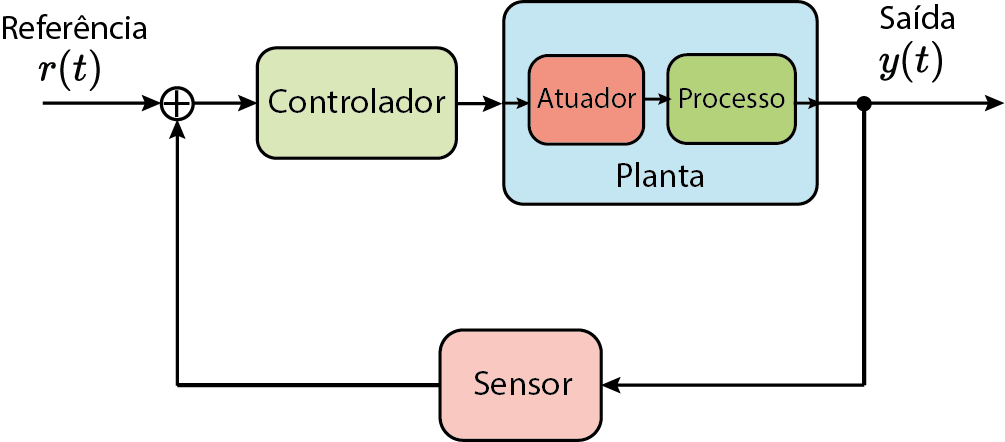
\includegraphics[width=0.72\linewidth]{malha_controle_atuador_processo.png}
    \caption[Próximos passos]{Na próxima aula (Projeto de Controladores ---
    Parte 2) detalha-se a malha considerando explicitamente atuador e processo,
    aprofundando os métodos de sintonia (LGR e Bode) no plano $z$.}
    \label{fig:proxima}
\end{figure}

\end{document}
